%!TEX root = ../thesis.tex
%*******************************************************************************
%****************************** Second Chapter *********************************
%*******************************************************************************

\chapter{Conclusions}\label{chap:summary}

\ifpdf
    \graphicspath{{Chapter7/Figs/Raster/}{Chapter7/Figs/PDF/}{Chapter7/Figs/}}
\else
    \graphicspath{{Chapter7/Figs/Vector/}{Chapter7/Figs/}}
\fi

\section{Summary and discussion}

This thesis has discussed the topic of dense 3D animal reconstruction from monocular images and video, using 3D morphable models as a strong prior over the object category. To this end, \Cref{chap:relwork} has covered the necessary technical background and related work, focusing particularly on the design of articulated models and methods for fitting them to input data. The core technical chapters have focused on three important considerations of particular importance to 3D animal tracking. 

\Cref{chap:cgas} contributes to perhaps the two most pertinant questions when reconstructing animals, namely (a) how to deal with the lack of 3D training data and (b) how to avoid the need for user intervention. The strategy for overcoming this involves using a 3D animal graphics model to generate training data for a deep learning pipeline. Consideration is given to various mechanisms for bridging the so-called `synth-to-real domain gap', but settles with a key observation that silhouettes are extremely informative to animal shape and pose and are simple to synthesize. In addition, silhouettes have become simple to extract from test set RGB sequences, by harnessing large training datasets generally designed for instance segmentation tasks. However, the chapter acknowledges that ambiguities exist when working in the silhouette domain, and proposes an optimal joint assignment discrete optimization problem, solved using quadratic programming and optimized using genetic algorithms, to try and recover the most likely skeleton trajectory over a video sequence. As is shown experimentally, the recovered trajectories are sufficient as input to a model fitting pipeline, which optimizes the SMAL~\cite{xxx} 3D morphable model to match this input evidence. 

However, despite success on these sequences, the approach has certain downsides. As demonstrated in \Cref{chap:wldo}, the quality of predicted joints at test time is heavily dependent on the quality of the shape and pose prior for generating varied shapes. This results in suboptimal performance on uncontrolled ``in-the-wild'' datasets of challenging shapes and poses, such as varied dog images sourced on the internet which are outside the range of the prior. Further, the approach is too slow to process video in real-time, which inhibits applications which could otherwise report behaviour anomalies in animals. These issues are tackled with the WLDO approach in \Cref{chap:wldo}. Firstly, a new 3D morphable model is designed with new limb scaling parameters and a more representative 3D shape prior is learnt during the training loop of a neural network. The method operates in real-time, and shows state-of-the-art performance on StanfordExtra, a new challenging dataset introduced in this chapter with no energy minimization phase necessary. The lack of 3D training data is overcome by means of a weakly supervised training strategy, making use of 2D annotations present in the training dataset.

Although WLDO is somewhat capable of handling images with some occlusion, similar to state-of-the-art approaches designed for 3D human reconstruction, heavily ambiguous input images cause failures. As explored, even when these networks are fine-tuned with such examples, they are restricted to recovering only a single possible reconstruction obtained by `averaging' over the space of plausible reconstructions. \Cref{chap:3dmulti} explores this problem and proposes to output a set of plausible reconstructions consistent with the input. Ambiguities in humans and animals are represented again using 3D morphable models. A multi-hypothesis network is trained using a best-of-$M$ loss. The chapter overcomes theoretical limitations with this construction, proposing a quantizer weighted by a normalizing flow prior to allow optimal sets of different sizes to be recovered without the need to entirely retrain the network. In additon, a 2D reprojection loss is used to discourage mode degeneration and ensure consistency to the input evidence. This approach is the first to specifically model ambiguities in an animal category and also achieves state of the art performance on competitive human benchmarks. Importantly, results are also demonstrated on RGBD-Dog, the first publically-available animal dataset with 3D annotations available for training and evaluation.

\section{Applicability to industrial animal tracking}

Many of the tools and techniques presented in this thesis have already found applications in industries strongly connected to animal husbandry. In particular, leading healthcare companies have made use of these technologies as part of their commitment to the 3Rs principles which apply when conducting pre-clinical trials of candidate medications that involve animals. Integrating continuous and automated animal monitoring systems to these studies helps \emph{R}efine the quality of collected data, which leads to an overall \emph{R}eduction to the number of animals required for each trial to produce results of scientific significance. This project, and others like it, also support the development of computerised behavioural models which could one day \emph{R}eplace the use of animals altogether.

For reasons of data privacy and confidentiality, results and images for this projects cannot be released in this thesis. However, permisison has been granted to allow a discussion of the methodology including some implementation details. 

A priority development area involves the WLDO system, presented in \Cref{chap:wldo} of this thesis. However, the system as demonstrated is restricted to producing 3D reconstructions of only a single animal. In addition, there has so far been no attention given to important downstream tasks, which are required by animal experts to enable prediction of animal behaviours and identities. This section will cover adaptations made to WLDO that enable its use in multi-housed animal environments, and a discussion on how to obtain per-animal behavioural output from 3D morphable model parameters.

%  The basis of research for this project has therefore been to extend WLDO to operate on multi-housed animals and to implement the downstream task, which outputs behaviours and identities. These components are handled in the subsequent sections:

 \subsection{Extending WLDO to multi-animal tracking}
 
 For reasons of animal welfare, it is preferable that animals in captivity should be housed in groups rather than in isolation~\cite{xxx}. To achieve this, it is necessary to adapt WLDO to support tracking and 3D reconstruction of multiple animals simultaneously. Inspired by recent work in object detection, WLDO has been implemented on top of an existing RCNN architecture. The components here are mostly standard: an input image is processed by a region proposal network (RPN) and region of interest (ROI) aligner to pass bounding object features to the later prediction heads. The WLDO layers which output 3D morphable model parameters are implemented as a new head, alongside existing heads which produce animal class ID (e.g. dog, cat etc.) and bounding box coordinates. Weights for existing layers (e.g. backbone and existing heads) are initialized using the MaskRCNN network trained on the MSCOCO dataset. This has the effect of making the core architecture proficient at identifying certain animal cateogries (i.e. up to the prediction heads) are initialized during the MaskRCNN network, pretrained on MSCOCO. This has the efficient that the core architecture is already proficient at detecting animal bounding boxes and identifying the species type at the start of training. Weights for the entire network (including those for the WLDO prediction head) are optimized by training on an internal dataset which have manually annotated segmentations and keypoints. With this architecture, the multi-animal WLDO network is capable at producing 3D reconstructions for all detected animals in the scene.

 \subsection{Predicting behaviours and identities}
 
 To meet the needs of veterninary experts, it is important to track individual animal behaviours throughout pre-clinical trials. Achieving this aim is hoped to contribute to a package of existing processes used to reveal insights around efficacy and potential risks associated with candidate medications. However, for reasons of ethics, it is discouraged to use physical markers on animals due to the risk of increased stress so the system should not rely on these for identification. Finally, the system should work continuously and therefore must operate on grayscale night vision images.

 The identity prediction is implemented as an additional prediction RCNN head which outputs an identity ID. For this reason, at present it is necessary to fine tune the weights of this branch for different animal subjects. Work is in progress to replace this module with an embedding space, learnt from multiple subjects, which can be used to discriminate between identities with only a few examples. The behaviour prediction module is implemented as a linear layer, mapping the parameters for the 3D morphable model to behaviour labels. This works effectively with only a fairly small network since all background information,texture and camera variation have already been solved for. 

 The modules are trained on a dataset collected internally over two days from 8 HD cameras with infrared night vision support. Labelling was conducted by in-house veterinary and clinical experts. Training the full system takes approximately 24 hours on a single V100 GPU. A system architecture diagram is given in \Cref{fig:dogdetectron}.

% PICTURE

\begin{figure}[t]
    \setlength{\fboxsep}{0pt}%
    \setlength{\fboxrule}{0pt}%
    \centering{\begin{tabular}{@{}c@{}}
        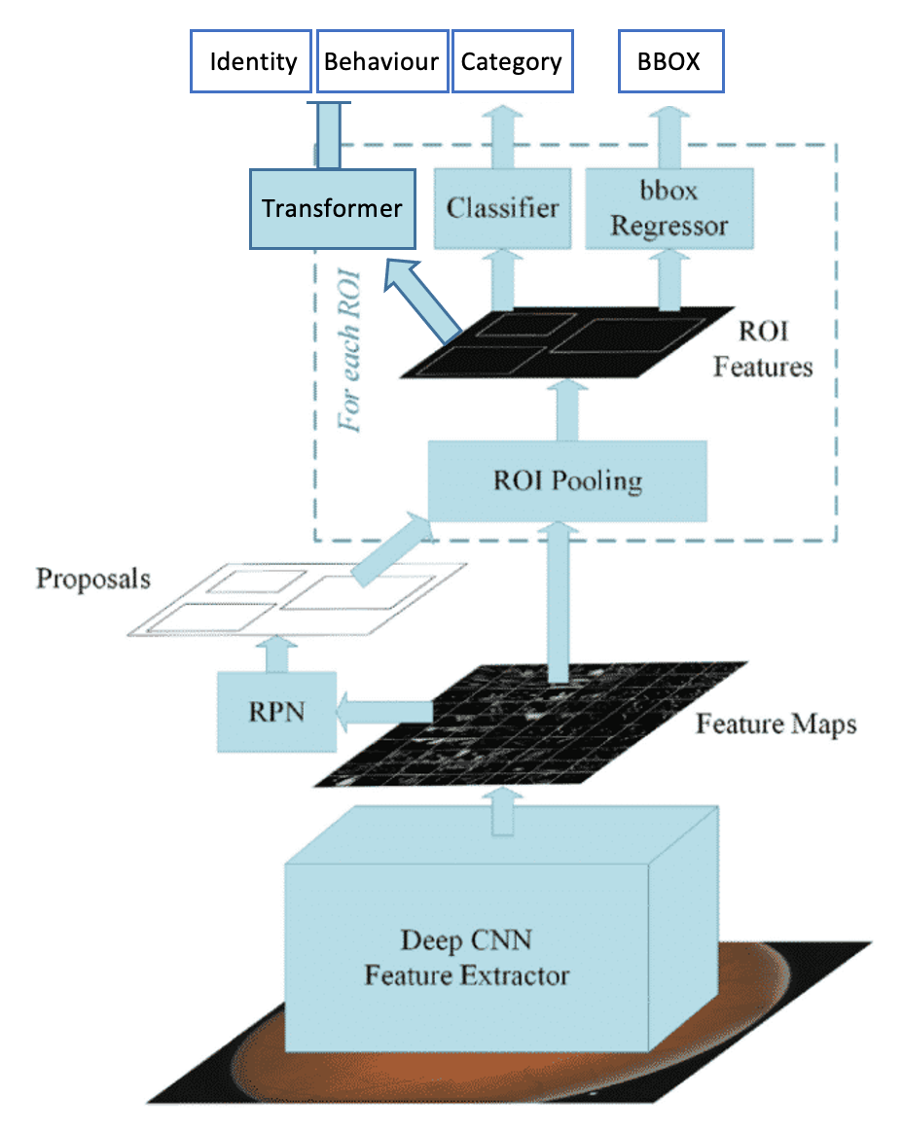
\includegraphics[width=0.99\linewidth]{dogdetectron.png}
    \end{tabular}}
    \captionof{figure}{
    \textbf{DogDetectron.}\label{fig:dogdetectron}
    }
    \end{figure}
    

\section{Discussions and areas for future work}

This final section of this thesis discusses the emerging field of 3D animal reconstruction as a whole with a view towards worthwhile avenues for further research.

\subsection{Representations of articulated 3D structures}

This thesis has used a popular category of 3D morphable models based on triangular meshes rigged with internal skeleton. Triangle meshes are a popular choice for representating 3D surfaces and particularly for articulated structures, as methods can take advantage of established deformation constraints such as linear blend skinning. In addition, compared to alternatives (e.g. voxel grids, OctNets, point clouds etc.) the representation is compact and easy to render. Mesh vertices (and linear combinations of them) are also useful constructs in order to determine correspondences between the 3D model and other modalities, particularly images. Minimizing the distance between projected mesh locations and image keypoints is an important loss used frequently in this thesis. 

However, the use of triangle meshes as 3D morphable models have some limitations, particularly when modelling detailed 3D surfaces or representing a large class of animal species.

\subsubsection{Implicit surface representations}

Although coarse animal shapes are easily represented~\cite{} uising a mesh structure, high frequency surface details (e.g. facial details, fur etc.) can only be captured with a large number of triangles and vertices. This necessitates an extremely complex mesh which becomes difficult for optimizers to fit, incurs a large memory footprint and slows down training and inference.

As discussed in \Cref{ss:implicit}, Neural Radience Fields (NeRF) are a relatively new class of implicit functions which are particularly adept at compactly representing high frequency details in complex 3D scenes. Starting with novel view synthesis on static scenes, there has been considerable progress in existing the formulation to video, generalizing to new environments, and most related to this thesis, operating on deformable 3D objects. 

At the time of writing, successful examples have been demonstrated on full humans and some body part categories (e.g. hands) but not yet for animal subjects. Part of the reason for this is likely the lack of large-scale 3D animal datasets which are typically required (but not always~\cite{xxx}) for training. 

% https://arxiv.org/pdf/2104.03953.pdf SNARF, ANerf
% Animatable Neural Radiance Fields for Human Body Modeling

While some NeRF approaches~\lazycite{}{NPMs, Multi-view NHR} learn human articulation from large-scale pose datasets (e.g. AMASS [30], DeformingThings4D [26], CAPE [30], MANO [45]), some maintain an internal 3D skeleton structure and focus NeRF at modelling complex skin/clothing features relative to these landmarks~\lazycite{xxx}{SNARF, ANerf, Animatable Neural Radience Fields}. Such an strategy could form the basis for an approach for animals, perhaps using WLDO in~\Cref{chap:wldo} to obtain a 3D animal skeletons and camera parameters and using an implicit representation to model the skin details. An interesting research direction here is to test if the implicit representation could be supervised by silhouettes alone.

If achieved, such a representation could enable facial features, skin abrasions, fur and other complex features to be incoporated. If recovered in images and video sequences of real animals, these details could be of considerable therapeutic significance. However, for real-world applications, consideration should be taken to ensure fast rendering at inference time. Until recently~\cite{xxx}, this has been a commonly cited concern with neural representations, which have typically required slow processes such as marching cubes. In addition, care must be taken when planning to use neural representations in a pipeline with a later downstream task, e.g. behaviour prediction. It is not immediately clear how to pass features from such a representation to subsequent classifiers; of course, one could pass network weights as input but these may be too complex or noisy a learning signal for effective behaviour prediction. However, animal shape could be modelled with sufficient precision, such a feature vector could be discriminative enough to use directly for animal identity -- potentially enabling single-shot recognition of different animals in multi-housed (or even wildlife~\lazycite{camera trap}{} scenarios.)

% implicit methods and incurs a large memory footprint that slows training and inference. 

% However, there are a recent class of implicit methods have been shown to be particularly adept at compactly representing high frequency details. As briefly discussed in ~\Cref{chap:relwork}, the idea is to represent the surface \emph{as} a neural network. For example, consider a network $f: \R{3} \mapsto \mathbb{B}$ which maps 3D locations to a binary occupancy value. The network outputs $1$ for 3D locations within the mesh and $0$ otherwise. Even higher quality results can be obtained by incorporating camera viewing direction into the input vector and outputing RGB values on top of occupany; with such a formulation, complex appearance details such as lighting and reflectance can be captured. 

% The class of Neural Radience Fields (NeRF) have produced impressive results on static scenes and have recently been extended to video~\cite{} and deformable categories. A common recent approach for modelling humans is to start by predicting a 3D skeleton (e.g. using SPIN~\cite{}) and allowing the implict function to represent the skin relative to the joints. However, these approaches require full 3D supervision of watertight meshes and have yet to show strong results on challenging input images.

% At present, implicit functions have not yet been applied to modelling animal categories, perhaps due to the increased challenge in capturing the full range of pose and shape diversity. However, research in this direction may lead to models being able to fully capture details such as fur, skin abrasions and other factors potentailly of therapeutic significance. 

% although attempts to model articulated objects  them to modelling objects with articulation is restricted to relatively simple cases. For example, the PIFu uses an implicit representation of humans and even captures clothing, but requires full 3D training data for training and results are shown only on humans captured in simple environments, poses and camera viewing directions. 

% works only in simple cases. However, while implicit functions are adept at representing static scenes, they struggle without these kind of implicit functions are non-structured, and are without an internal skeleton, therefore they struggle to model articulation. Further, these approaches typically require large 3D datasets of watertight meshes for training. 

% There are some recent works which aim to represent articulated 3D structures with implicit functions. A popular approach is to first predict an internal skeleton and use the implicit function to represent the ``skin''. This seems a promising approach; reducing the need for large datasets to learn pose and instead focusing the network on it's primary job to capture surface details.
% Neural Parametric Models for 3D Deformable Shapes

% Rendering is also slow... but say there has been work on this.

% However, despite representing being adept at representing the coarse structure of an animal, meshes are inefficient when needing to represent high frequency surface features, particularly when such features are unknown in advance. For large scale scenes, meshes are a poor choice due to the need to  

% Two problems; (1) you need lots of triangles to represent details, (2) you can't distribute triangles as needed. 

% Complain about the fidelity of reconstruction, difficultly representing fine-grained features. 

% Introduce implicit representations. Then complain they are useless at articulated strucutres. It's of course possible to try and learn a deformation space from examples, but such work is dififcult and relies on a large dataset of examples.
% We need articulated Nerf which contains an internal skeleton.

\subsubsection{Modelling the animal kingdom}

% Introduce automatic rigging, and structured shape representations which can gain and lose features. 

The technical chapters of this thesis have covered methods for reconstructing a range of diverse animal species, including humans, dogs, camels, tigers, cats and more. However, apart from humans as a special case, despite being of varying shapes the remaining animals all have similar topology. In particularly, they have a common internal skeletal structure which includes precisely four legs and a tail. This holds true in recent animal reconstruction literature; methods are either designed for a single species using a specially designed template model~\lazycite{}{AWF dolphins} or cover a small range of species with common topology. However, it is natural to question whether a 3D reconstruction system could be designed to cover this full range; including less common animal classes. 

Of course, a simple way of tackling this would be to design dozens of 3D morphable models with a defined shape space for each animal type. An object detector could then be used to identify which to apply to each input image. However, this would be a laborious exercise and would not take advantage of common features between different types. Zuffi et al.~\lazycite{3dmen}{} have already exploited this for quadrupeds by demonstrating the SMAL linear shape space is capable of modelling pigs and other species not present in the training data. Some progress has been made in the direction of modelling out-of-domain species, by incoporating a free-form vertex optimization step after an initial SMAL fit to allow reconstruction of appendages out of the training domain, e.g. an elephant's trunk or reindeer's horns. However, the idea of building a unified model which can represent quadrupeds alongside animals of entirely different topology (e.g. whales, ducks, snakes) remains largely unexplored. \Cref{fig:animalkingdom} shows an example of these categories. 

\begin{figure}[t]
\setlength{\fboxsep}{0pt}%
\setlength{\fboxrule}{0pt}%
\centering{\begin{tabular}{@{}c@{}}
    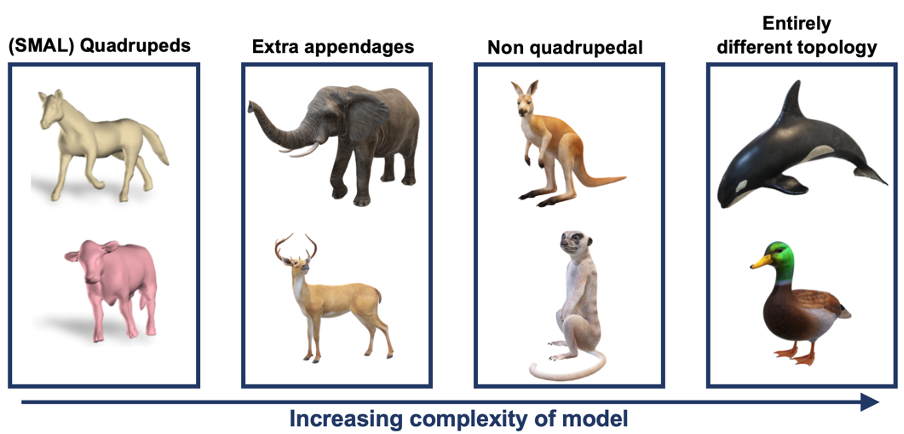
\includegraphics[width=0.99\linewidth]{increasing_model_complexity.png}
\end{tabular}}
\captionof{figure}{
\textbf{Examples of challenging animal categories.}\label{fig:animalkingdom}
}
\end{figure}


\begin{figure}[t]
\setlength{\fboxsep}{0pt}%
\setlength{\fboxrule}{0pt}%
\centering{\begin{tabular}{@{}c@{}}
    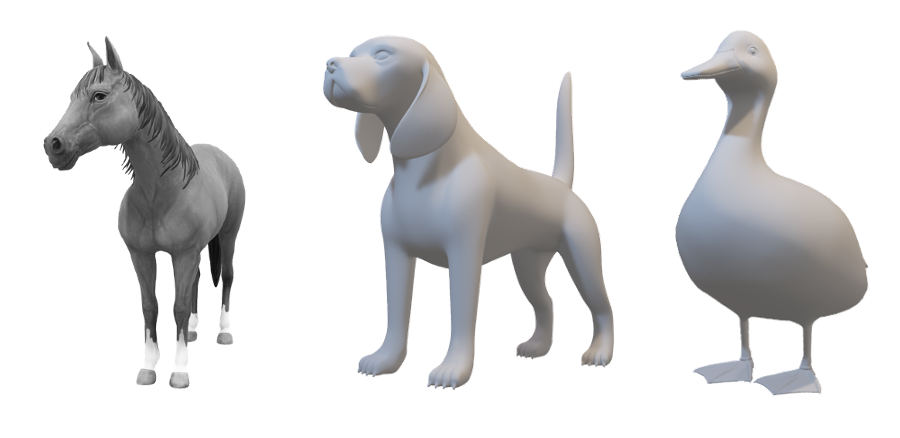
\includegraphics[width=0.99\linewidth]{synthetic_animalkingdom.png}
\end{tabular}}
\captionof{figure}{
\textbf{Examples of challenging animal categories.}\label{fig:synthetic_animalkingdom}
}
\end{figure}
    

There are two possible approaches to handling this challenge. The first avenue of exploration is to look at techniques which operate without a 3D morphable model at all, overcoming the need to design one for each individual species. As discussed in \Cref{chap:relwork} implicit methods~\lazycite{}{PIFu} have shown results on a simple animal category (humans) under constrained camera viewpoints but rely on full 3D supervision. Other work~\lazycite{}{CMU or UCMU} replaces a 3D morphable model with a sphere, initialized to match the mean shape in the category (e.g. birds). Novotny et al. has demonstrated model-free 3D sparse keypoint reconstruction using only 2D training data, relying on deep neural network implementations of non-rigid structure from motion. They show sparse results on humans and dense results on other non-animal categories. However, techniques in this category are not yet able to perform with the quality and robustness of such techniques on articulated animal categories with images captured in the wild. However, these are interesting directions for future work.

% been designed for simpler categoriework on 3D humans, under constrained camera viewpoints mentioned before, there are implicit approaches for simpler poses~\lazycite{PIFu}{} which require full 3D training data and emerging approaches based requiring only 2D keypoints, for simpler animals such as birds (although strong initialization is still used)~\lazycite{}{Bird paper} and human keypoints~\cite{}{David's papers}. However, the quality and robustness of such techniques on in-the-wild and uncontrolled images are not yet comparable. However, these are worthy avenues of research.

% free-form vertex advantages are afforded by learning a shape space which can linear there is asystem could be designed  to  operateA natural question is to ask whether the approaches defined in this thesis would extend to different, stranger animal classes. For example, would WLDO work on an octupus? The hesitant answer to this is `yes' subject to having access to a representative 3D morphable model that matches the topology of the target species. With sufficient training examples, the initialized model should adapt using expectation maximization steps to better capture the species in question. However, given that there are 8.7 million different species of animal on Earth, it is clearly intractable to consider designing a 3D morphable model, complete with an internal skeleton and shape space for all of them.

An alternative approach would be to consider designing a more sophisticated 3D morphabel model that generalizes across a wide range of species. Clearly, a large dataset of 3D scans and exemplar poses are needed, but this can be sourced from online animation data (e.g. see ~\Cref{fig:synthetic_animalkingdom}). The challenge is then to consider learning a model that generalizes to all species. To achieve this, one could examine work that models structures with different internal structure or topology. For example, CoMA~\lazycite{}{CoMA} replaces conventional linear shape spaces by training a convolutional mesh autoencoder to represent faces. FoldingNet~\lazycite{}{FoldingNet} represents diverse furniture shapes by learning how to warp an input 2D grid to create the 3D structure. More recently, StructureNet~\lazycite{}{StructureNet} generates 3D shapes with an internal graph network capable of modelling different parts to discourage gaps in the output. All of these techniques could be employed to represent the various shapes of animals. \Cref{fig:foldingnet} shows an example of FoldingNet trained on various animal categories and reconstructions of unseen test examples. Note the model works well on quadrupeds alonside a salmon fish. This line of work is interesting and is worthy of further research.

\begin{figure}[t]
\setlength{\fboxsep}{0pt}%
\setlength{\fboxrule}{0pt}%
\centering{\begin{tabular}{@{}c@{}}
    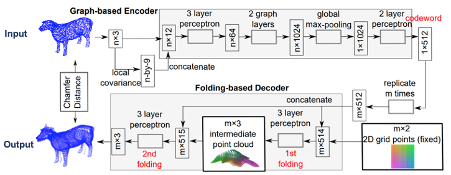
\includegraphics[width=0.99\linewidth]{foldingnet-example.png} \\
    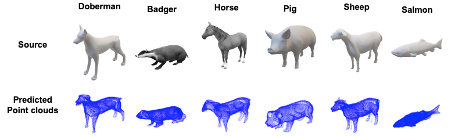
\includegraphics[width=0.49\linewidth]{foldingnet-results.png}
    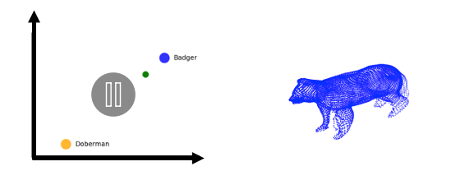
\includegraphics[width=0.49\linewidth]{foldingnet-interp.png}
\end{tabular}}
\captionof{figure}{
\textbf{Examples of challenging animal categories.}\label{fig:foldingnet}
}
\end{figure}


% idesigning a more sophisticated morphable model which extends to all species. much more representative shape prior by training on the plethora of 3D artist data or even obtaining scans from museums. 

% unconare still far behind  and attempts to template-free approaches for humans in simpler capture environments, attempts at extending non-rigid structure from motion methodologies for humans this for humans~\cite{PiFu}, static objects There have been early attempts at this,  For this reason, it is proposed that a worthy area of investigation is to design 

% fall into a category of ``medium-to-large quadruped'' thesis, attention has been given to reconstruction 

% and OctTrees and as-rigid-as-possible come with a long history of as they are compact and easy to render. ParticulaSpecifically for articulated structures, techniques benefit from established deformation constraints such as linear blend skinning to ensure plausible surface variations. 


% In this thesis, meshes have been integrated into neural network architectures by fixing the triangulation according to a 3D morphable model and outputting vertex locations parameterized by shape and pose. 


% are a suitable choice for modelling articulated structures, as reconstruction techniques can make use of established deformation constraints, such as  including linear blend skinning, as-rigid-as-possible deformation constraints, differentiable rendering and others. Additionally,  for this work, due to a long history of work in 


% However, it is not clear how to design a 3D morphable model to cover groups of animals with considerably different topologies. an appropriate does not naturally extend when representing animals with considerably different topologies; for example, consider modelling an octupus, dog and marmoset. In such a case, it is necessary 

% In addition, methods can take advantage of a long history of methods for meshes, many covered in \Cref{chap:relwork} of this thesis including differentiable rendering, linear blend skining, ARAP regularizers and many more etc. 

% For representing articulated structures, meshes are more appropriate than voxel grids, in which a surface is represented as occupany values over a fixed sized 3D grid. For this reason, the resolution of the output surface scales cubicly in the size of the grid, most of which is usually sparse. Improvements to this have recently been made with OctNets~\cite{xxx}, which use octrees~\cite{xxx} to learn a more efficient partitioning of the voxel space, thereby reducing memory. 

% However, 

% neural   and are an appropriate choice for neural networks; sinceoffering a fixed set of vertices a 3D surface a representation has some benefits; for example, the such a representation has some limitations. triangular meshes rigged with internals as the 
% representation for  

% \begin{enumerate}
%     \item Use of radiance fields. PiFu and Nerf. etc.
%     \item Represented thousands of different animals. Shape modelling from structured chairs interpolation paper.
% \end{enumerate}


\subsection{Modelling reconstruction ambiguity}

% Normalizing flows 
% Shape modelling (difficult with SMPL, easier with implicits)
% Enable training sets and calibrated confidences for animal exports


\Cref{chap:3dmulti} of this thesis focuses on modelling natural ambiguities present when reconstructing articulated objects, particularly from images exihibiting occlusion. In part due to limitations in the availability of 3D datasets with sufficient shape variation (e.g. RGBD-Dog contains a few dogs and 3D human datasets notoriously underrepresent people of different body sizes), the focus of this chapter was to model ambiguities in reconstructed pose. This was explored through generating multiple hypotheses using a min-of-$M$ loss and developing a quantizer based on normalizing flow weighting to retrieve an output set of optimal size. However, modelling shape is of particular importance to animal categories and is a worthy direction for extending these intial ideas. 

The presentation in \Cref{chap:3dmulti} could be trivially extended to model shape, firstly by generating $M$ shape predictions, one for each hypothesis rather than sharing a single one. The normalizing flow could model shape by allowing shape parameters to influence the 3D locations used for training rather than working in the shape-normalized space. Similar ideas (although based on Mixture Density Networks) have since been explored by Sengputa et at.~\lazycite{}{Ignas paper}. However, since these models are based on linear shape spaces so are the ambiguities. This causes difficulty when trying to model the shape ambiguities across the reconstructed 3D surface. This limitation would be avoided with a different shape representation, for example implicit functions or other shape spaces as discussed in the previous section.

Finally, authors may look to developing research into normalizing flows. In this thesis, these relatively new architectures have been employed as 3D pose priors but researchers could be more ambitious. For example, one may train a direct mapping between 3D morphable model parameters (e.g. shape and pose) and a gaussian space. Experimentally, it was found that the RealNVP model struggled to model the complex relationship in shape and pose parameters but perhaps improved pipelines would fair better. If realised, this would allow the full distribution (complete with likelihoods) to be expressed over the 3D morphable model.

% could model shape by  hypotheses rather than a single one alongside the Due to limitations in available datasets, the focus of this work was in modelling variations in poses. For example, RGBD-Dog contains only shape for a few dog categories and 3D human datasets are notoriously unrepresentative of different human shapes. For animals, modelling ambiguities in sahthere has been some recent work which specifically creates a dataset of 3D shape from 3D shape dataset from   do in part due to the limited availability of 3D datasets with significant variation in shape (e.g. RGBD ) data the focus of this chapter has been to 

\subsection{Generating synthetic animals}

\Cref{chap:cgas} of this thesis explores a methodology for generating synthetic animals from a graphics engine. The resulting dataset is then used to train a neural network to predict 2D keypoints. In this chapter, a key insight is to bridge the synth-to-real domain gap by training on synthetic \emph{silhouette} images and testing on silhouettes extracted from real data (either automatically or by hand). However, as acknowledged, while silhouettes are strongly informative over the 3D shape, there remain ambiguities that require additional machinery (e.g. the optimal joint assignment method) to resolve.

There has been a great deal of recent work focuses on generating high quality synthetic data. Generative Adversarial Networks (GANs) cast the task as a `competition' between two networks: the \emph{generator} network produces synthetic images and the \emph{discriminator} determines if a given input image originated in a real-world dataset or was instead synthesized by the generator. These two networks are given opposite goals: the generator is penalized if it fails to `fool' the discriminator, and the discriminator is penalized if it fails to recognize a synthesized image. By training these networks jointly, the generator eventually learns to produce synthetic images of extremely high quality, since the discriminator provides feedback on even subtle aspects of the synthetic images which are unreaslistic. 

Despite the remarkable quality of `GANerated' images, applying these networks to generate 3D synthetic animals for the purpose of generating a training dataset is non trivial. Popular applications of GANs are in ``noise-to-image'' translation tasks, for example to generate synthetic artworks which appear similar to work by a famous painter, or ``image-to-image'' tasks, such as colorizing greyscale photography. The difficulty with such approaches is they are \emph{unstructured}. For the methods in this thesis, it is not enough to just generate a synthetic dataset of realistic-looking animals; rather, it is critical that the underlying 3D structure (e.g. 2D keypoints, 3D parameters) is known in order to ground truth for learning. 

To achieve this, a natural approach is to task a generator with synthesizing realistic UV texture maps which can be applied to colourize a 3D morphable animal model. SMAL parameters could then be sampled as in \Cref{chap:cgas}, a synthetic texture map applied and then differentiably rendered on a random background (for example, as used in 3D-Safari~\lazycite{}{3d safari}). The discriminator could compare these output images to a distribution of real-world animal images, and propagate error back to the generator. Such an approach should theoretically result in realistic synthetic images with internal contours since these are present in the real dataset. These can then be used later on for disambiguating limbs. However, there are a number of challenges with such an approach. Firstly, the rendering pipeline has no ability to construct fur, clothing, objects or accessories (e.g. collars) which occur systematically in the real-world data distribution. In addition, the pipeline is thought to produce artefacts, particularly when alpha blending with random backgrounds. These issues cause a problem when training, as the discriminator can lock onto such features to solve its problem, but as the generator has no control over the full rendering pipeline (only the input texture map), it cannot learn from this feedback. 

% accersizthe challenge of such an approach is the rendering pipeline creates artefacts which  is that arfacts caused by differentiable rendering on top of random backgrounds ontop ofthis approach is that a differentiable rendering piepline cannot hope to synthesize all of the necessary components of a natural looking input image. Firstly, synthetizithe rendering pipeline has no means to create backgroundsgenerate accessories (e.g. collars, clothing), fur or other objects fur,  creates arfeis known to create artefacts renders often create cannot hope to synthesize all the necessary components of a natural looking input image. Firstly, the system has no means to create backgrounds and creating blurring differentiable rendering pipelines create artefacts which the discriminator locks on to but the generator cannot fix, since it is only able to affect the input texture map. 

% A large dataset of real world animal images could be used as the target distribution. As in \Cref{chap:cgas}, sampling parameters for this model and rendering (this time, textured) images could then be used for training. However, it was found experimentally that this approach does not bridge the domain gap; the likely cause is that the rendering engine creates artefacts which the discriminator can lock on to, solving its task trivially. Since the generator has no control over the rendering pipeline, it cannot learn from this feedback.

\subsubsection{Painting by numbers: a 3D animal GAN}

Therefore, an alternative approach gives the generator full control over the rendering pipeline. The idea is to create images by sampling pose and shape parameters of the morphable model and rendering from a random camera viewpoint.A generator is then use to add `realism' to this render, adding details that make the image appear as if from a distribution of real images. However, in this process, it is very important that the generator does not corrupt the pose, shape nor camera parameters when adding detail, or otherwise the image will no longer match the parameters later used for ground truth. 

This is achieved with a simple idea, inspired by the Vitruvian Manifold~\lazycite{}{VM} and DensePose~\lazycite{}{DP}. A special texture map of surface locations is applied to the morphable model. Each SMPL surface point is assigned a tuple $(x,y,z)$ which refers to the 3D location on SMPL model in its canonical T-pose. Note that an alternative parameterization $(s,u,v)$ where $s$ is the surface part ID and $(u,v)$ refers to a location on the unwrapped 2D parameterization as in DensePose could be used as an alternative.

Similar to the presentation in ~\Cref{chap:cgas}, random pose $\pose$, shape $\shape$ and positioning parameters $\posn$ are sampled. The texture map of canonical locations is applied and a renderer is used to generate a synthetic image. A generator function then maps from the image of canonical SMPL coordinates to an RGB image $g: \mathbb{R}^{H \times W \ times 3} \mapsto \mathbb{R}^{H \times W \ times 3}$ to convert the image of canonical SMPL coordinates to an RGB image. A PatchGAN~\lazycite{}{PatchGAN} discriminator $d: \mathbb{R}^{H \times W \ times 3} \mapsto \mathbb{R}^{H' \times W'}$ takes either an image produced by the generator, or a image from the real dataset and predicts a measure of realism, expressed as a value between 0 and 1.

A native implementation of the generator $g$ leads to the architecture successfully creating realistic looking humans, but they do not match the pose and shape of the initial render. This is because there is no incentive for the network for preserve these characteristics in the detail generating phase. This is overcome by setting up the generator to have only a few layers where each has a small receptive field. By doing this, the generator has an insufficient receptive field size to create a complete and realistic looking human to fool the discriminator which has a larger receptive field and can therefore check for such problems. However, the generator can solve this task by taking advantage of the canonical SMPL coordinates rendered on the initial image. 

The generator therefore learns to create a continuous mapping, from canonical SMPL coordinates to RGB values. In essence, the function learns to assign a colour to each SMPL coordinate, which can be thought of as designing a texture map for the character. By doing this well, the generator can create realistic looking humans by only needing to consider each pixel independently of the rest. Another analogy is to think of this as `painting by numbers': the initial rendering indicates an $(x,y,z)$ canonical coordinate and the network colours this in appropriately.

Another advantage of this formulation is that by allowing a small but \emph{non-zero} receptive field, the model is capable of learning appearance details slightly beyond the boundaries of the SMPL character. Therefore, clothing and floor details systematic in the input images can be generated, allowing the discriminator and generator to continue learning. 

% https://github.com/benjiebob/cvpr2021_gan/blob/b95e2627fadbdcaf66891bc72d78d05bab2c255b/dp_gan/networks/gan/gan.py#L361
% https://github.com/benjiebob/cvpr2021_gan/blob/b95e2627fadbdcaf66891bc72d78d05bab2c255b/dp_gan/networks/gan/gan.py#L784

The network is tested using Subject 1 from Human3.6M to see if it is capable of assigning human-like texture features to rendered SMPL images. Results can be seen in Figure XXX.

\begin{figure}[t]
    \setlength{\fboxsep}{0pt}%
    \setlength{\fboxrule}{0pt}%
    \centering{\begin{tabular}{@{}c@{}}
        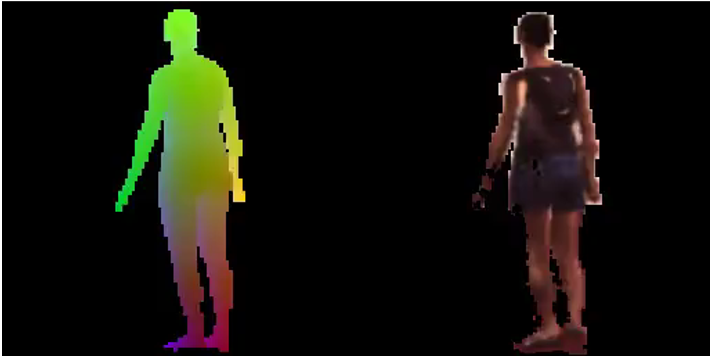
\includegraphics[width=0.99\linewidth]{humangan.png}
    \end{tabular}}
    \captionof{figure}{
    \textbf{Human GAN.}\label{fig:humangan}
    }
    \end{figure}
    

Of course, this is only a part solution. Further work in this direction is required to extend this technique to be able to generate different subjects in different clothing, subsequently train a network to recover the 3D parameters from the output of the generator and test on real images. Eventually, since no real 3D data (or even 2D data except silhouettes) is required for training, the network could be trained and tested on animal subjects. 

Note that despite promising results on humans, the network heavily relies on good quality 3D shape and pose priors for sampling synthetic characters. As discussed in \Cref{chap:cgas}, these are not easily obtainable for animals. It is thought that this approach would operate well on simpler animals in standard poses (e.g. Grey's zebras~\lazycite{}{3d safari}) but would still struggle without better priors on more challenging datasets such as StanfordExtra. However, as discussed above, better priors could perhaps be obtained using animation data for example.

\subsection{Large-scale animal datasets for evaluation}

A major constraint to methods working on 3D animal reconstruction is the lack of suitable datasets for evaluating methods. Due to this, the general field must evaluate the quality of 3D models on real world data using 2D metrics. As in \Cref{chap:cgas} and \Cref{chap:wldo} of this thesis, these are obtained by projecting the 3D model to a 2D image and computing Probability of Correct Keypoint (PCK) using ground truth 2D keypoints or Intersection over Union (IoU) using the ground truth 2D silhouette. Particularly since these metrics are computed from the same viewing direction as the captured image they do not evaluate the quality of the reverse side of the 3D structure. However, reconstruction errors are more likely to occur on the `invisible' part of the subject. 

These factors have been mitigated in this thesis using synthetic data and producing detailed qualitative results for examination by the reader. However, as the field develops, large-scale 3D evaluation datasets will be required to to enable fast hyperparameter sweeps and to compare the quality of different methods. 

Some progress has been made with RGBD-Dog~\lazycite{}{RGBDog}, the first available animal dataset with 3D annotations. However, the scale of the dataset is limited to 7 dogs which are captured in specialised clothing in a single environment. Future work should aim to capture a range of animals performing a number of different poses. 

\subsection{Improved use of video for motion priors and force analysis}

\Cref{chap:cgas} introduces a simple temporal prior used to encourage a smooth motion trajectory over the input video sequence to improve the quality of reconstruction. Future work could improve this by learning a more detailed model of animal motion over a video, perhaps taking advantage of the typical limb patterns characteristic to particular species. With such modelling, perhaps more challenging video datasets (e.g. dog shows, horse racing) would become possible for reconstruction. 

For applications in biomechanical analysis, after recovering the animal 3D structure there is great potential in modelling forces through the body. Such insights could help diagnose joint problems, such as arthritis. Additionally, since many animals are in a known environment (e.g. zoos), techniques developed for humans which simultaneously reason about the subject and environment would be interesting to apply to animals. 

% \section{Broader impact}

% Our method improves the ability of machines to understand human body poses in images and videos.
% Understanding people automatically may arguably be misused by bad actors.
% However, importantly, our method is \emph{not} a form of biometric as it does \emph{not} allow the identification of people.
% Rather, only their overall body shape and pose is reconstructed, but these details are insufficient for unique identification.
% In particular, individual facial features are not reconstructed at all.

% Furthermore, our method is an improvement of existing capabilities, but does not introduce a radical new capability in machine learning.
% Thus our contribution is unlikely to facilitate misuse of technology which is already available to anyone.

% Finally, any potential negative use of a technology should be balanced against positive uses.
% Understanding body poses has many legitimate applications in VR and AR, medical, assistance to the elderly, assistance to the visual impaired, autonomous driving, human-machine interactions, image and video categorization, platform integrity, etc.



